\section{The Model}

\frame
{
	\begin{center}
		\LARGE The Model: Evolution of Mimicry
	\end{center}
}

\frame
{
	\frametitle{The Model}
	\framesubtitle{Evolution of Mimicry}
	
	\begin{itemize}
		\item \textbf{Objective:} Build an \textit{agent based} Artificial Life model for simulating the evolution of mimicry.	
		\item Two species of agents:
			\begin{enumerate}
				\item Prey
					\begin{itemize}
						\item Model
						\item Mimic
					\end{itemize}
				\item Predator
			\end{enumerate}
		\item Prey pattern representation: Cellular Automata.
		\item Predator pattern recognition: Hopfield Network.
		\item Environment: Visual representation, 3D, toroidal.
	\end{itemize}	
}

\subsection{Past Work}

\frame
{
	\frametitle{The Model}
	\framesubtitle{Past Work}

	\begin{itemize}
		\item Turner(1996) and Huheey(1988):
			\begin{itemize}
				\item \textbf{Focus:} Selective pressure on prey, by learning ability of predator.
				\item Predators use simple Monte Carlo learning or mathematical approach.
			\end{itemize}
		\item Sherratt(2002):
			\begin{itemize}
				\item Co-evolving predator and prey population.
				\item Predators are deterministic, cannot learn from experience.
				\item Predators attack policy is fixed, either attack or avoid.
			\end{itemize}
	\end{itemize}
}

%-------------------------------
%More slides on Franks and Noble
%-------------------------------

\frame
{
	\frametitle{Past Work}
	\framesubtitle{Franks and Noble}

	\begin{itemize}
		\item First Model(2002):
			\begin{itemize}
				\item \textbf{Focus:} 
				\item Predators use simple Monte Carlo learning or mathematical approach.
			\end{itemize}
		\item Second Model(2004):
			\begin{itemize}
				\item Co-evolving predator and prey population.
				\item Predators are deterministic, cannot learn from experience.
				\item Predators attack policy is fixed, either attack or avoid.
			\end{itemize}
	\end{itemize}
}

%-------------------------------
%More slides on Franks and Noble
%-------------------------------

\subsection{FormAL}

\frame
{
	\frametitle{FormAL Framework}
	
	\begin{itemize}
		\item Ideas from Peter Grogono's Formal Artificial Life (FormAL) project.
		\item \textbf{Goal:}		
			\begin{itemize}
				\item To study the emergence of complexity.
				\item No variable unless genetically controlled or influenced. \textit{Principal not followed for Hopfield Network.}
			\end{itemize}
		\item \textbf{Agents:}
			\begin{itemize}
				\item Simulated organism.
				\item Able to reproduce itself using genetic information.
				\item Capable of modifying structures of genome between generations.
				\item Able to interact with other agents.
				\item Survive and reproduce in a challenging environment.
			\end{itemize}
	\end{itemize}
	
}

\frame
{
	\frametitle{FormAL Framework}
	\framesubtitle{Environment}
	
	Environment is 3D, where agents get complete freedom of movement defined from genetic representation.
	\begin{itemize}
		\item \textbf{Space:}
			\begin{itemize}
				\item 
			\end{itemize}
		\item \textbf{Time:}
			\begin{itemize}
				\item 
			\end{itemize}
		\item \textbf{Cell:}
			\begin{itemize}
				\item 
			\end{itemize}
	\end{itemize}
}

\frame
{
	\frametitle{FormAL Framework}
	\framesubtitle{Environment Parameters}
	
	\begin{table}[H]
	\centering
	\begin{spacing}{1.5}
	\begin{scriptsize}
%	\begin{tabular}{| p{2.2cm} | >{\centering} p{3cm} | p{7.5cm} |}
	\begin{tabular}{| p{1.5cm} | >{\centering} p{2cm} | p{4cm} |}
		\hline
			\textbf{Parameter} & \textbf{Value} & \textbf{Description} \\ \hline
			ISize & 6 & Number of cell in single dimension of the 3-D toroidal cube\\ \hline
			World Size & 20 & Size of a single dimension of the 3-D toroidal cube\\ \hline
			Cell Size & \( World Size / ISize \) & Size of each cell\\ \hline
			Total Number of Cells & \( ISize^3  = 216\) & Total number of cells in the environment\\ 
		\hline
	\end{tabular}
	\end{scriptsize}
	\end{spacing}
	\caption{Parameters to control the environment.}
	\label{tab:environment-control-parameters}
	\end{table}
}

\frame
{
	\frametitle{FormAL Framework}
	\framesubtitle{Environment - Visual representation - Front}

	\begin{figure}[H]
		\centering
		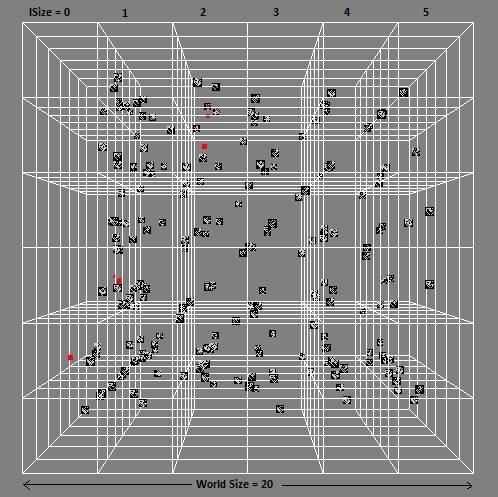
\includegraphics[scale=0.40]{../tex/images/cells-front}
		\caption{Three dimensional representation of the environment divided in cells. Presence of different species of agents inside.}
	\label{tab:3-d-environment-images-1}
	\end{figure}	
}

\frame
{
	\frametitle{FormAL Framework}
	\framesubtitle{Environment - Visual representation - Top}

	\begin{figure}[H]
		\centering
		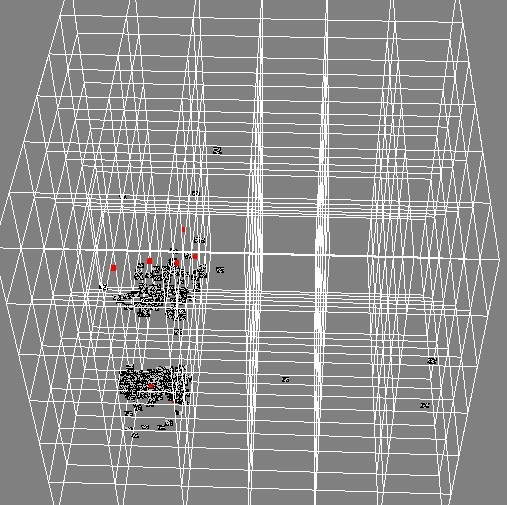
\includegraphics[scale=0.40]{../tex/images/cells-top}
		\caption{Three dimensional representation of the environment divided in cells. Presence of different species of agents inside.}
	\label{tab:3-d-environment-images-2}
	\end{figure}	
}

\frame
{
	\frametitle{FormAL Framework}
	\framesubtitle{Environment - Visual representation - Side}

	\begin{figure}[H]
		\centering
		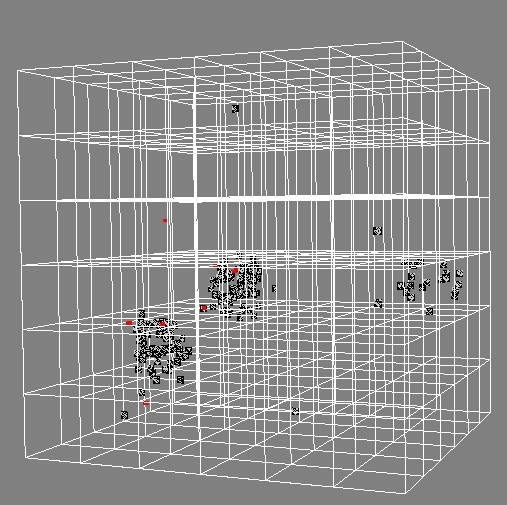
\includegraphics[scale=0.40]{../tex/images/cells-side}
		\caption{Three dimensional representation of the environment divided in cells. Presence of different species of agents inside.}
	\label{tab:3-d-environment-images-3}
	\end{figure}	
}

\frame
{
	\frametitle{FormAL Framework}
	\framesubtitle{Agent Mobility}
	
	\begin{itemize}
		\item 
	\end{itemize}

}

\frame
{
	\frametitle{FormAL Framework}
	\framesubtitle{Mobility Parameters}

	\begin{table}
	\centering
	\begin{scriptsize}
	\begin{spacing}{1.5}
	\begin{tabular}{| p{1.3cm} | >{\centering} p{1cm} | p{5cm} |}
		\hline
			\textbf{Parameter} & \textbf{Value} & \textbf{Description} \\ \hline
			Force Factor & 40 & A unit vector is multiplied by this amount before being added to the force vector.\\ \hline
			Differential Time Step (DT) & 0.01 & The time step used for first-order integration of the motion equations.\\ \hline
			Friction & 5 & The friction constant used for motion calculations.\\ \hline
			Work Factor & 1 & \( Work done = WF * force * distance \), where \(WF\) is this constant.\\
		\hline
	\end{tabular}
	\end{spacing}
	\end{scriptsize}
	\caption{Parameters to control mobility of agents.}
	\label{tab:mobility-control-parameters}
	\end{table}
	
}

\subsection{Prey}

\frame
{
	\frametitle{The Prey: Mimics and Models}
	\framesubtitle{Pattern Representation}
}

\frame
{
	\frametitle{The Prey: Mimics and Models}
	\framesubtitle{Species Diversity}
}

\frame
{
	\frametitle{The Prey: Mimics and Models}
	\framesubtitle{Genome}
	
	\begin{table}[H]
	\centering
	\begin{scriptsize}
	\begin{spacing}{1.5}
	\begin{tabular}{|c|c|c|c|}
		\hline
			\textbf{Pattern(8)} & \textbf{Palatability(2)} & \textbf{Mobility(6)} & \textbf{Reproduction(1)} \\ \hline
			10101101					 	& 							01		 		 & 			110001					&					1						 		 \\ \hline
	\end{tabular}
	\end{spacing}
	\end{scriptsize}
	\caption{Distribution and purpose of each gene of the 17 bit prey genome.}
	\label{tab:prey-genome}
	\end{table}
}

\frame
{
	\frametitle{The Prey: Mimics and Models}
	\framesubtitle{Punctuated Equilibrium}
}

\frame
{
	\frametitle{The Prey: Mimics and Models}
	\framesubtitle{Palatability: Genomic Representation }
}

\frame
{
	\frametitle{The Prey: Mimics and Models}
	\framesubtitle{Interaction: other prey}
}

\frame
{
	\frametitle{The Prey: Mimics and Models}
	\framesubtitle{Interaction: predators}
}

\frame
{
	\frametitle{The Prey: Mimics and Models}
	\framesubtitle{Mobility}
}

\frame
{
	\frametitle{The Prey: Mimics and Models}
	\framesubtitle{Reproduction}
}

\frame
{
	\frametitle{The Prey: Mimics and Models}
	\framesubtitle{Configuration Parameters}
	
	\begin{table}[H]
	\centering
	\begin{scriptsize}
	\begin{tabular}{| p{1.5cm} | >{\centering} p{1cm} | p{4cm} |}
		\hline
			\textbf{Parameter} & \textbf{Value} & \textbf{Description} \\ \hline
			Prey Size & 2 to 5 & Size of the prey species in the 3D FormAL  environment.\\ \hline
			Reproduction age limit & 100 & Minimum number of iterations or time steps a prey species need to be present in the simulation to get reproduction capability\\ \hline
			Reproduction interval & 1000 & Number of iterations a prey need to wait before reproducing again.\\ \hline
			Pattern Mutation Rate & 0.05 & Rate of Mutation of the pattern genome.\\ \hline
			Genome Mutation Rate & 0.5 & Rate of mutation of the rest of the genome excluding the pattern gene.\\ \hline
			Demise Age & 2000 & Age at which the prey species will be removed from the environment.\\
		\hline
	\end{tabular}
	\end{scriptsize}
	\caption{Parameters to control prey population and visibility.}
	\label{tab:prey-control-parameters}
	\end{table}
}

\subsection{Predator}

\frame
{
	\frametitle{The Predator}
}